\chapter{Fenster}
\renewcommand{\chaptertitle}{Fenster}

\lehead[]{\sf\hspace*{-2.00cm}\textcolor{white}{\colorbox{lightblue}{\makebox[1.60cm][r]{\thechapter}}}\hspace{0.17cm}\textcolor{lightblue}{\chaptertitle}}
\rohead[]{\textcolor{lightblue}{\chaptertitle}\sf\hspace*{0.17cm}\textcolor{white}{\colorbox{lightblue}{\makebox[1.60cm][l]{\thechapter}}}\hspace{-2.00cm}}
%\chead[]{}
\rehead[]{\textcolor{lightblue}{AvHG, Inf, My}}
\lohead[]{\textcolor{lightblue}{AvHG, Inf, My}}

\lstset{style=myJava}

\section{Klassen-Hierarchie in AWT und Swing}

\begin{minipage}{0.45\textwidth}
Wer in Java grafische Benutzerschnittstellen (GUI) programmieren will hat die
Wahl zwischen AWT und Swing. Sowohl AWT (\myPackage{java.awt.*}) als auch Swing
(\myPackage{javax.swing.*}) sind als Bibliotheken Teil jeder Java Runtime
Environment (JRE) – stehen also auf allen Systemen, die Java anbieten zur Verfügung.

Swing ist etwas moderner und bietet auch mehr Funktionalität. Wir werden uns
deshalb auf Swing konzentrieren. Aus dem (stark vereinfachten) Klassendiagramm
rechts kann man erkennen, dass man auch bei der Swing-Programmierung nicht ohne
AWT auskommt, da die Swing Klassen aus AWT-Klassen abgeleitet sind.

Swing-Klassen erkennt man an dem führenden 'J' im Klassennamen. Wie etwa
\myClass{JLabel} oder \myClass{JMenu}.


\begin{compactitem}
\item[\myClass{java.awt.Component}]\hfill
  \begin{compactitem}[$\bullet$]
  \item abstrakte Klasse
  \item ein „GUI-Element“ mit Größe und Position
  \item kann Ereignisse senden und darauf reagieren  
  \end{compactitem}
\end{compactitem}

\end{minipage}
\hfill
\begin{minipage}{0.5\textwidth}
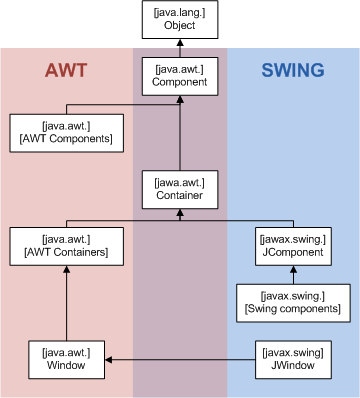
\includegraphics[width=1.0\textwidth]{./inf/SEKII/23_Java_Frames/AWTSwingClassHierarchy.png}
% http://commons.wikimedia.org/wiki/File:AWTSwingClassHierarchy.png
% Public Domain
\end{minipage}

\begin{compactitem}
\item[\myClass{java.awt.Container}]\hfill
  \begin{compactitem}[$\bullet$]
  \item abstrakte Klasse
  \item kann andere Komponenten aufnehmen
  \item Positionierung und Anordnung von Dialog Elementen in Zusammenarbeit mit
  LayoutManager-Klassen
  \end{compactitem}

\item[\myClass{javax.swing.JFrame}]\hfill
  \begin{compactitem}[$\bullet$]
  \item Hauptfenster (Top-Level-Fenster) mit Rahmen und Titelleiste
  \item optionales Menü
  \item dem Fenster kann ein Icon zugeordnet werden
  \item Aussehen der Maus kann verändert werden
  \end{compactitem}

\item[\myClass{javax.swing.JWindow}]\hfill
  \begin{compactitem}[$\bullet$]
  \item Hauptfenster (Top-Level-Fenster) ohne Rahmen, Titelleiste und Menü
  \item Anwendung übernimmt das Zeichnen der Rahmen selbst
  \end{compactitem}

\item[\myClass{javax.swing.JDialog}]\hfill
  \begin{compactitem}[$\bullet$]
  \item Hauptfenster (Top-Level-Fenster) zum Anzeigen von Dialogen
  \end{compactitem}

\item[\myClass{javax.swing.JPanel}]\hfill
  \begin{compactitem}[$\bullet$]
  \item einfachste konkrete Ableitung von JComponent und Container
  \item wird verwendet, um eine Sammlung von Dialog-Elementen mit einem
  vorgegebenen Layout zu definieren
  \end{compactitem}

\end{compactitem}


Als Merksatz: Die Hauptfenster-Klassen aus Swing sind direkt aus den
entsprechenden Hauptfenster-Klassen des AWT abgeleitet. Alle anderen
Swing-Klassen leiten sich aus \myClass{JComponent} ab.

Für uns von besonderer Bedeutung sind zunächst die Klassen \myClass{JFrame} und
\myClass{JPanel}. Unsere Anwendungsfenster leiten wir aus der Klasse
\myClass{JFrame} ab. Um innerhalb eines Frames Komponenten wie Buttons oder
Textfelder positionieren zu können, brauchen wir aber zunächst einen Container,
der diese Komponenten aufnehmen kann. Genau dies leistet \myClass{JPanel}.


\section{Erstellung eines eigenständigen Java-Programms}

Ein eigenständiges Programm muss die folgende Methode besitzen, die beim
automatisch Programmstart aufgerufen wird:

\begin{lstlisting}
public static void main(String[] args)
\end{lstlisting}


\section{Erzeugung eines Programmfensters}

Es muss eine eigene Klasse von der Klasse \myClass{JFrame} abgeleitet werden.
Dabei ist folgendes zu beachten:

\begin{compactenum}[1.]
\item \myClass{JFrame}-Objekt erzeugen

\item Mit der \myClass{JFrame}-Methode \lstinline|setDefaultCloseOperation()|
wird definiert, was beim Schließen des Fensters geschehen soll. Wir verwenden
hier typischerweise \lstinline|JFrame.EXIT_ON_CLOSE| als Argument.

\item Einen Container (\myClass{JPanel}) erzeugen und auf der sogenannten
„contentPane“ platzieren.

\item Komponenten hinzufügen und/oder mit \lstinline|paintComponent()| zeichnen.

\item \myClass{JFrame}-Methode \lstinline|setVisible(true)| macht das Fenster
sichtbar.
\end{compactenum}


\section{Methoden von \myClass{JFrame} (Auswahl)}

\bgroup
\def\arraystretch{1.2}
\begin{tabularx}{\textwidth}{|X|p{80mm}|}
\hline
\lstinline|JFrame()|\linebreak\lstinline|JFrame(String title)| &
im Konstruktor kann der Titel angegeben werden
\\ \hline
\lstinline|void setSize(int width, int height)| &
setzt die Fenstergröße in Pixeln
\\ \hline
\lstinline|void setLocation(int x, int y)| &
Positioniert das Fenster. Angegeben wird die linke obere Fensterecke in Pixeln.
Position (0, 0) ist die linke obere Ecke des Monitors.
\\ \hline
\lstinline|void setVisible(boolean b)| &
macht das Fenster sichtbar oder unsichtbar
\\ \hline
\lstinline|void setTitle(String title)| &
verändert den Titel des Fensters
\\ \hline
\lstinline|void repaint()| &
Das System löscht den Bildschirm und ruft dann die
\lstinline|paintComponent()|-Methoden der betroffenen Komponenten auf
\\ \hline
\end{tabularx}
\egroup


\section{Fenster-Ereignisse}

\bgroup
\def\arraystretch{1.2}
\begin{tabular}{ll}
Mögliche Ereignisquellen: \hspace{15mm} &
\myClass{JWindow}, \myClass{JDialog}, \myClass{JFrame}
\\
Registrierungsmethode: &
\lstinline|void addWindowListener(WindowListener l)|
\\
Interface für Empfänger: &
\myClass{WindowListener} \hspace{10mm} [Adapterklasse: \myClass{WindowAdapter}]
\hfill \\
\end{tabular}
\egroup

\subsection{Methoden des Interfaces \myClass{WindowListener}}

\bgroup
\def\arraystretch{1.2}
\begin{tabular}{|l|l|}\hline
\lstinline|void windowOpened(WindowEvent e)| &
Fenster wurde geöffnet
\\ \hline
\lstinline|void windowClosing(WindowEvent e)| &
Fenster soll geschlossen werden
\\ \hline
\lstinline|void windowClosed(WindowEvent e)| &
Fenster wurde geschlossen
\\ \hline
\lstinline|void windowIconified(WindowEvent e)| &
Fenster wurde auf Symbolgröße verkleinert
\\ \hline
\lstinline|void windowDeiconified(WindowEvent e)| &
Fenster wurde wiederhergestellt
\\ \hline
\lstinline|void windowActivated(WindowEvent e)| &
Benutzer arbeitet jetzt in dem Fenster
\\ \hline
\lstinline|void windowDeactivated(WindowEvent e)| &
Benutzer arbeitet nicht mehr in dem Fenster
\\ \hline
\end{tabular}
\egroup

\subsection{Wichtige Methode von WindowEvent}

\bgroup
\def\arraystretch{1.2}
\begin{tabular}{|l|l|}\hline
\lstinline|Window getWindow()| &
gibt das Fenster zurück, in dem das Ereignis passierte
\\ \hline
\end{tabular}
\egroup


\section{Beispiel}

\begin{lstlisting}[numbers=left, xleftmargin=7mm]
import java.awt.*;
import javax.swing.*;
import javax.swing.border.EmptyBorder;

public class MyJFrame extends JFrame {
    æ// globale Variablen
æ    private static final int WIDTH = 500;
    private static final int HEIGHT = 500;
    private static final Color BACKGROUND = Color.WHITE;
    private static final Color FOREGROUND = Color.BLACK;
    private JLabel zeichenflaeche;

    public MyJFrame(final String title) {
        super(title);
        setDefaultCloseOperation(JFrame.EXIT_ON_CLOSE);
        JPanel contentPane = new JPanel();
        contentPane.setBorder(new EmptyBorder(5, 5, 5, 5));
        contentPane.setLayout(new BorderLayout(0, 0));
        setContentPane(contentPane);
        zeichenflaeche = new JLabel() {
            @Override
            protected void paintComponent(Graphics g) {
                super.paintComponent(g);
                myPaint(g);
            }
        };
        zeichenflaeche.setPreferredSize(new Dimension(WIDTH, HEIGHT));
        zeichenflaeche.setOpaque(true);
        zeichenflaeche.setBackground(BACKGROUND);
        zeichenflaeche.setForeground(FOREGROUND);
        zeichenflaeche.setFont(new Font("Arial", Font.PLAIN, 12));
        contentPane.add(zeichenflaeche);
        pack();
        setLocationRelativeTo(null);
        setResizable(false);
        setVisible(true);
    }

    public void myPaint(Graphics g) {
        // wird aufgerufen, wenn das Fenster neu gezeichnet wird
        g.drawString("Guten Tag!", 100, 200);
    }

    public static void main(final String[] args) {
        EventQueue.invokeLater(new Runnable() {
            public void run() {
                try {
                    MyJFrame anwendung = new MyJFrame("MyJFrame");
                } catch (Exception e) {
                    e.printStackTrace();
                }
            }
        });
    }
}
\end{lstlisting}

\subsection{Erläuterungen zum Beispiel}

\begin{compactitem}
\item[Zeile 14:] Im Konstruktor wird zunächst der Konstruktor der Super-Klasse
(\myClass{JFrame}) aufgerufen. Der Titel des Fensters wird übergeben.

\item[Zeile 15:] Hier wird festgelegt, dass das Programm beendet werden soll,
sobald der Benutzer den Schließen-Knopf des Fensters benutzt.

\item[Zeile 16-17:] Ein \myClass{JPanel}-Container wird mit Rahmen erzeugt.

\item[Zeile 18:] Der LayoutManager für diesen Container wird bestimmt.

\item[Zeile 19:] Der Container wird als contentPane benutzt.

\item[Zeile 20-26:]  Ein neues \myClass{JLabel}-Objekt wird erzeugt. Die
\lstinline|paintComponent()|-Methode der \myClass{JLabel}-Klasse wird dabei
überschrieben, so dass es nun möglich ist beliebige Zeichenoperationen auf
dieser Komponente auszuführen (ausgelagert in die Methode \lstinline|myPaint()|,
die in den Zeilen 39-42 definiert wird).

\item[Zeile 27:] Die Größe des neuen \myClass{JLabel}-Objekts (nicht die des
Fensters!) wird festgelegt.

\item[Zeile 28:] Die Deckkraft des \myClass{JLabel}-Objekts wird eingestellt.
\lstinline|true| bedeutet, dass das Objekt deckend gezeichnet wird. Mit
\lstinline|false| würde es durchsichtig gezeichnet.

\item[Zeile 29-31:] Vorder- und Hintergrundfarbe sowie der verwendete Font
werden eingestellt.

\item[Zeile 32:] Das \myClass{JLabel}-Objekt wird auf der contentPane plaziert.

\item[Zeile 33:] Mit \lstinline|pack()| wird die Größe des Fensters so gesetzt,
dass alle Komponenten darin den nötigen Platz finden. (Hinweis:
\lstinline|pack()| macht nur Sinn, wenn ein LayoutManager benutzt wird! Da ihr
auch des öfteren ohne LayoutManager arbeiten werdet, wird es bei euch auch oft
Beispiele geben, in denen \lstinline|pack()| nicht benutzt wird).) 

\item[Zeile 34:] Das Fenster wird in der Bildschirmmitte geöffnet.

\item[Zeile 35:] Es kann durch den Anwender nicht in seiner Größe verändert
werden.

\item[Zeile 36:] Jetzt erst wird das fertige Fenster auf dem Desktop angezeigt.

\item[Zeile 44-55:] In der \lstinline|main()|-Methode unseres Programms wird der
Konstruktor unseres Anwendungsfensters innerhalb eines
\lstinline|try-catch|-Blocks in den sogenannten Event Dispatch Thread (EDT)
eingestellt.
\end{compactitem}


\section{\myClass{WindowListener} verwenden}

Statt es uns einfach zu machen und wie in Zeile 15 des Beispielprogramms auf
die gegebene Funktionalität von Swing zurückzugreifen, können wir auch selbst
dafür sorgen, dass das Schließen des Fensters durch den Benutzer auch
tatsächlich zur Beendigung des Programms führt.

Dazu erzeugen wir zunächst eine neue Klasse \myClass{FensterSchliesser}, die wir
von der Klasse \myClass{WindowAdapter} ableiten:

\begin{lstlisting}
import java.awt.*;
import java.awt.event.*;

class FensterSchliesser extends WindowAdapter {
    public void windowClosing (WindowEvent event) {
        MyJFrame frame = (MyJFrame) event.getWindow();
        frame.setVisible(false);
        frame.dispose();
        System.exit(0);
    }
}
\end{lstlisting}

Und ersetzen anschließend Zeile 15 in unserem Beispiel durch:

\begin{lstlisting}
    setDefaultCloseOperation(JFrame.DO_NOTHING_ON_CLOSE);
    FensterSchliesser close = new FensterSchliesser();
    addWindowListener(close);
\end{lstlisting}


\section{Auf das Objekt des Anwendungsfensters zugreifen}

Die Methode \lstinline|getWindow()| gibt ein Objekt der Superklasse
\myClass{Window} zurück:

\begin{lstlisting}
Window w = event.getWindow();
\end{lstlisting}

Solange man mit dem Datentyp \myClass{Window} arbeitet, kann man jedoch nur auf
Variablen und Methoden zugreifen, die in der Klasse \myClass{Window} definiert
sind.

Wenn man auf Variablen und Methoden zugreifen möchte, die in abgeleiteten
Klassen definiert sind (z.B. eine Variable, die man selbst in seinem eigenen
Anwendungsfenster definiert hat), muss man den Datentyp umwandeln. Das geht so:

\begin{lstlisting}
MeinFrame frame = (MeinFrame) w;
\end{lstlisting}


\section{Programmierung von komplexen Dialogen}

Ein allgemeiner Dialog wird ganz ähnlich programmiert wie ein Frame. Der
Haupt-Unterschied ist, dass man seine eigene Klasse nicht von der Klasse
\myClass{JFrame} sondern von der Klasse \myClass{JDialog} ableitet. Darüber
hinaus sind folgende Details zu beachten:

\begin{compactitem}
\item In einem Dialog gibt es natürlich keine \lstinline|main()|-Methode, da der
Dialog nicht wie das Anwendungsfenster vom System selbst gestartet wird. Der
Code, der beim Frame zur Erzeugung des Objektes in der
\lstinline|main()|-Methode steht, wird in den Event-Handler gepackt, der beim
Klick des entsprechenden Buttons im Hauptfenster aufgerufen wird (Näheres dazu
im nächsten Kapitel).

\item Im Konstruktor sollte mit der Anweisung \lstinline|super()| der folgende
Konstruktor der Superklasse Dialog aufgerufen werden:

\begin{lstlisting}
public Dialog(Dialog owner, String title, boolean modal)
\end{lstlisting}

Für \lstinline|modal| übergibt man den Wert \lstinline|true| um einen
sogenannten {\em modalen Dialog} zu erzeugen. Bei einem modalen Dialog kann der
Benutzer das Hauptfenster nicht benutzen solange der Dialog geöffnet ist.

\item Wie im Frame muss das Event \lstinline|windowClosing| abgefangen werden,
um das Fenster zu schließen. Während beim Frame jedoch die komplette Anwendung
geschlossen wird (\lstinline|EXIT_ON_CLOSE|) darf bei einem Unterdialog nur das
aktuelle Fenster geschlossen werden:

\begin{lstlisting}
dialog.setDefaultCloseOperation(JDialog.DISPOSE_ON_CLOSE);
\end{lstlisting}
\end{compactitem}
